%\chapter{Methodology}
\label{chap:chapter3}

\section{Dataset and MySQL Database}
\label{sec:dataset_db}

\subsection{Dataset}
The dataset contains all information that is currently available in the StackExchange community 
(at the time the dataset was created). The following is a list of the tables found in the dataset:
\begin{itemize}
	\item Badges: Badges awarded to users.
	\item Comments: Comments given either to a question or an answer.
	\item Posts: Posts on StackExchange, this contains both questions and answers.
	\item Posthistory: The history of a given post (e.g. edits, reason for closing, etc.).
	\item Postlinks: Link to other Posts (e.g. duplicates).
	\item Users: Information about the given user registered at the given community.
	\item Votes: Type of vote given to a Post (e.g. up/down, vote to close, etc.).
\end{itemize}
In the beginning, the dataset that was used was downloaded in August 2015. However, since this turned out 
to be outdated, the latest dataset was downloaded from (\url{https://archive.org/details/stackexchange}) on 
30. March 2016. The dataset comes in zip-files, where each zip-file contains all the rows found in the given 
 table. These rows are presented in an XML file, as shown in Listing \ref{lst:so_xml_file}.
% listing
\begin{lstlisting}[caption={Content in stackoverflow.com-Tags.xml}, label={lst:so_xml_file}] 
<?xml version="1.0" encoding="utf-8"?>
<tags>
<row Id="1" TagName=".net" Count="227675" ExcerptPostId="3624959" 
WikiPostId="3607476" />
<row Id="2" TagName="html" Count="511091" ExcerptPostId="3673183" 
WikiPostId="3673182" />
...
</tags>
\end{lstlisting}

\subsection{MySQL Database}
In the beginning, the issue was getting access to the file and see how it looked like. Since most of these XML 
files had a large file size (ranging from 3,9 MB to 71,9 GB) none of the editors could open them. Attempting to open 
them through Python code also failed, since there was not enough memory to process everything. The only solution 
was therefore to create a MySQL database that could contain all the data. 

Setting up the MySQL database was not a straight forward process. The operative system I was running was Arch 
Linux, where they had switched from using Oracle's MySQL to MariaDB\footnote{See 
	\url{https://wiki.archlinux.org/index.php/MySQL}.}. One of the main problems was the available storage 
space\footnote{The HDD with Arch Linux installed had a disk size of 500 GB, with four partitions; root, var, 
	swap and home. 40 GB was used for /root and /var, 12 GB was used for swap and the remainder was used for 
	/home.} and the varying file sizes. Some of the issues were mainly connection timeout, no more disk space 
and connection loss (e.g. "Error Code: 2013. Lost connection to MySQL server during query"). To avoid losing 
the connection to the database, the timeout values had to be changed in MySQL Workbench 
(shown in Figure \ref{fig:mysql_wb_settings}).

\begin{figure}[ht]
	\centering
	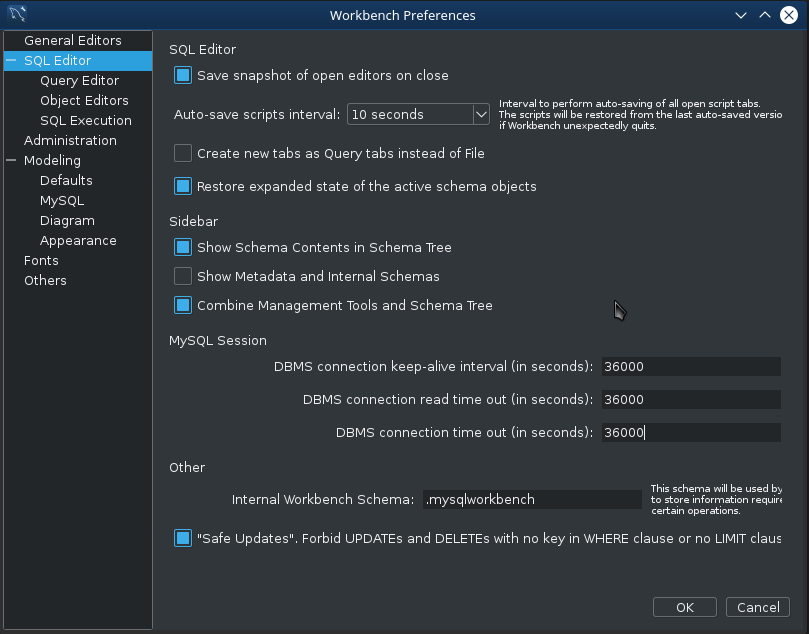
\includegraphics[width=0.6\textwidth]{mysql_wb_settings}
	\caption{MySQL Workbench: Setting timeout values to avoid connection loss}
	\label{fig:mysql_wb_settings}
\end{figure}

The next problem was the lack of disk space. MySQL by default stores all databases and belonging tables in 
 /var/lib/mysql/, and it also creates temporary backup files (where the file size is equal to the size of the 
 current database). Since the default folder for temporary files was on /root, the disk space was used up in 
 less than 30 minutes. Therefore, two things needed to be done. First, disable the storage of temporary files, 
 and secondly change the storage location for the database. The problem when tinkering with the configuration 
 file is that things easily break. Which is what happened, and a clean install was needed for both 
 MariaDB and MySQL (the changed settings can be seen in Listing  \ref{lst:mariadb_config_file}). The final step 
 was to create symbolic links that linked the database to the 
 location where the tables where stored (this has to be done before creating the tables, if not MySQL 
 Workbench will store the tables in /var/lib/mysql/)\footnote{It should be noted that after an upgrade of 
 	MariaDB, MySQL and MariaDB could no longer find the tables, even if they still were in the /home/mysql/ 
 	 folder. It is therefore advisable to dump the database after inserting all the tables, since it goes a lot 
 	 faster to restore the database from dump rather than insertion from XML files.}. 


\begin{lstlisting}[caption={Changes made to config file: /etc/mysql/my.cnf}, label={lst:mariadb_config_file}] 
# disable storage of temporary files
#tmpdir = /tmp/		  
# disable storage of log files
#log-bin = mysql-bin  

# set directory for storing database files
datadir = /home/mysql 
\end{lstlisting}

Listing \ref{lst:load_xml_file} shows how the files were loaded into the tables, and the complete database can 
be seen in Appendix \ref{app:mysql_database}, p.~\pageref{app:mysql_database}. Since the Posts table is large 
(\textasciitilde 29,5 million rows) and it contains both questions and answers, two new tables were created; 
"posvote\_Posts"\footnote{The Posts table has a file size of \textasciitilde 43,6 GB, whereas posvote\_Posts file 
	size is \textasciitilde 11,2 GB. negvote\_Posts has a file size of \textasciitilde 1,33 GB.} and 
"negvote\_Posts". posvote\_Posts contains questions with a score higher then zero (score > 0) and negvote\_Posts 
contains all questions with a score lower then zero (score < 0).

% Listing showing the SQL for loading XML row data into MySQL
\begin{lstlisting}[caption={Load XML file into a table in the MySQL database}, label={lst:load_xml_file}] 
LOAD XML LOCAL INFILE 
path_to_xml_file
INTO TABLE db_table
ROWS IDENTIFIED BY '<row>';
\end{lstlisting}

\section{Development process} 
\label{sec:libsvm_implementation}
When starting the development, most of the focus was on retrieving the data from the database, and being able 
to process it for text analysis. 

The main problem was that all the questions contained HTML, starting with the 
<p> tag, as shown in Listing \ref{lst:unprocessed_question}.

\begin{lstlisting}[caption={Question before processing (Question ID: 941156)}, label={lst:unprocessed_question}] 
<p>
Why do we need callbacks in ASP.NET or any server side technology?
</p>&#xA;&#xA;<p>One answer can be, to achieve asynchronous calls. 
</p>&#xA;&#xA;<p>But I am not satisfied with this answer.</p>
&#xA;&#xA;<p>Please explain it in a different way.
</p>
&#xA;
\end{lstlisting}


program development \\
issues with setting up environment, installations, etc \\
library choices: scikitlearn, pandas, bs4, etc \\
implementation of scikit-learn \\
issues during development, etc \\
changed from aug to march dataset to get more data \\
switching from -10/+50 to -5/+50 to get more separation (and more results for bad) \\
switching from "good"/"bad" to +/-1 for class label (bcz libsvm)


\begin{comment}
	Timeline:
		1. Created retrieval method for bad questions from db
			1.1. Using pandas to store data retrieved from db
		2. Added HTML class to remove tags
			Source: http://stackoverflow.com/questions/753052/strip-html-from-strings-in-python
			Accepted answer: "answered May 29 '09 at 11:47 Eloff"
			And comment to this answer by 'pihentagyu aka James Doepp' (May 21 '15 at 17:49)
		3. Tutorial by: \url{http://radimrehurek.com/data_science_python/}
		4. Removal of codeblocks from the question
			4.1 Using BeatifulSoup to processes tags without end-tags			
			4.2 Issues with losing the tail (text after codeblock); attaching it to parent
			4.3 Issue "NoneType + str: TypeError". Caused by parent not having tail. 
				Fixed by adding a .tail and setting it to '' on the <parent>.
			4.4 HTML w/ XML causing issues; parser fails (because parser was also xml, adding xml 
				to beginning of text). Example: \url{http://stackoverflow.com/questions/19535331/print-page-specific-area-or-element}
			4.5 Filtering out questions that failed by adding their index to a temp list, and then 
				removing them from dataset
		5. Issue: Scikit-learn documentation is for v17.1, whereas I was using developer version v18.0
		   (part of the issue was that it wasn't installable, so it was installed from GitHub repo instead)
		   considered switching to libsvm (which wasn't installable through pypi in the beginning)
		6. Instead of removing codeblocks, the text 'has\_codeblock' was added to indicate code was used
			6.1 Stored the processed questions to .csv
		7. Discovered data missing in some questions by looking at the CSV. 
		   Some <code> snippetes weren't removed. Content found after EOF
		   Issue 4.4 was fixed by removing all lxml conversion and using bs4 instead
		8. Questions start with <p>, this was removed by setting all text to be on one line
		9. Removal of numeric and hexadecimal values from text. Issue with trash data, e.g:
			\url{http://stackoverflow.com/questions/856307/wordwrap-a-very-long-string}
		10. Trash data: Using NLTK, NLTK.WordNet and enchant
			10.1 Tested out WordNet, could not discover english words. Does not contain all english words
			10.2 Tested out enchant, but could not in all cases either discover all english words
			10.3 Using Porter stemming to reduce features
			10.? \url{http://www.irfanelahi.com/data-science-document-classification-python/#Lexical-
			Analysis-of-the-Text-Data}
			10.? Setting min\_df=0.01 (ignore those occuring in less then 1\%) - helped a lot 
		11. Stemming of data, model creation and gridsearch with SGD			
		12. Model based on 20,000 samples (10k good, 10k bad) - took approx ~3hours for both models
			Model 1 was for all data (no test set). Model 2 was based on train\_test\_split
		13. Added tags column to the used dataset. Added the unprocessed dataset (but html is removed)
		14. Tested out different SVM algorithms (SVC, SGD and LinearSVC)
			Issue was that I managed to overwrite the .csv, so I had to do everything over again
			took approximately 24-36 hours to complete (+ 3days before hand to make everything run smoothly).
		15. Attempted to use optparse, argparse to make it executable. 
			Problem is that it exits after command is run. Need it to continue running to be able to:
				a) create new (or load existing) model
				b) use model from a) to predict quality of entered question (rinse/repeat)
		16. Used while loop instead (loop until exit entered). shortcuts are the same as with argparse, but 
			without the '-' in front (e.g. instead of -e, just press 'e' to exit)
\end{comment}

\section{Feature sets, attributes and processing}
\label{sec:feature_sets}
what features were selected and why? \\
how was data processed (e.g. retrieved from db, converted to scikit-learn format, and so forth) \\
attributes: length, symbols, question sentence only, code snippet, votes, closed, etc.

